\documentclass[runningheads,a4paper]{llncs}

% Set TOC depth to 3
%\setcounter{tocdepth}{3}

% Package for change tracking
%\usepackage[disabled]{chgtrk}
%\usepackage{chgtrk}
%\newCTcontributor{Karla}
%\newCTcontributor{Colin}
%\newCTcontributor{Rob}
%\newCTcontributor{Son}
%\newCTcontributor{Michael}

% Package for typesetting AMS Symbols
\usepackage{amssymb}

% Package for typesetting abbreviations
\usepackage{abbrev-SCXMLREF}


% Package for typesetting diagrams using TikZ
\usepackage{tikz}
\usetikzlibrary{positioning}
%\usepackage{pgf-picture}

% Package for typesetting requirements
%\usepackage[compact]{reqdoc}

% Package for typesetting Event-B mathematical symbols
\usepackage{bsymb}

% Package for typesetting SCXMLREF example models in Event-B
%\usepackage{eventB-SCXMLREF}

% Package for AMS Math
\usepackage{amsmath}

% Package for typesetting URLs
\usepackage{url}
\urldef{\mailsa}\path|{cfs, t.s.hoang, mjb}@ecs.soton.ac.uk|
\urldef{\mailsa}\path|{knmorri, rob}@sandia.gov|

% package for fancy tables
\usepackage{booktabs}

% Package for highlight TODOs
%\usepackage[disable]{hltodonotes}
%\usepackage[]{hltodonotes}

\newcommand{\keywords}[1]{\par\addvspace\baselineskip
\noindent\keywordname\enspace\ignorespaces#1}

% Package for fancy references
\usepackage{varioref}

% Package for including figures
\usepackage{graphicx}
\usepackage{subcaption}

% Package for sub-floats (e.g. figures)
% \usepackage{subfig}

% Package for including standalone source files
\usepackage{standalone}

% For floating listings
\usepackage{float}
\newfloat{lstfloat}{htbp}{lop}
\floatname{lstfloat}{Listing}
\def\lstfloatautorefname{Listing} % needed for hyperref/auroref

% Package for listings (e.g. JavaScript)
%\usepackage{eventBlistings}

\usepackage{hyperref}
\hypersetup{
  colorlinks=true,
  linkcolor = blue,
  urlcolor=cyan!50!black,
  citecolor=cyan,
}

\usepackage{examplep}
% Package for typesetting Event-B, load this package after all other packages
\usepackage[colour]{lstEventB}

% Listing for XML
\definecolor{dkgreen}{rgb}{0,0.6,0}
\definecolor{gray}{rgb}{0.5,0.5,0.5}
\definecolor{mauve}{rgb}{0.58,0,0.82}
\definecolor{gray}{rgb}{0.4,0.4,0.4}
\definecolor{darkblue}{rgb}{0.0,0.0,0.6}
\definecolor{lightblue}{rgb}{0.0,0.0,0.9}
\definecolor{cyan}{rgb}{0.0,0.6,0.6}
\definecolor{darkred}{rgb}{0.6,0.0,0.0}

\lstset{
  basicstyle=\ttfamily\scriptsize,
%  basicstyle=\ttfamily\footnotesize,
  columns=fullflexible,
  showstringspaces=false,
  numbers=left,                   % where to put the line-numbers
  numberstyle=\tiny\color{gray},  % the style that is used for the line-numbers
  stepnumber=1,
  numbersep=5pt,                  % how far the line-numbers are from the code
  backgroundcolor=\color{white},      % choose the background color. You must add \usepackage{color}
  showspaces=false,               % show spaces adding particular underscores
  showstringspaces=false,         % underline spaces within strings
  showtabs=false,                 % show tabs within strings adding particular underscores
  frame=none,                   % adds a frame around the code
  rulecolor=\color{black},        % if not set, the frame-color may be changed on line-breaks within not-black text (e.g. commens (green here))
  tabsize=2,                      % sets default tabsize to 2 spaces
  captionpos=b,                   % sets the caption-position to bottom
  breaklines=true,                % sets automatic line breaking
  breakatwhitespace=false,        % sets if automatic breaks should only happen at whitespace
  title=\lstname,                   % show the filename of files included with \lstinputlisting;
                                  % also try caption instead of title  
  commentstyle=\color{gray}\upshape
}

\lstdefinelanguage{XML}
{
  morestring=[s][\color{mauve}]{"}{"},
  morestring=[s][\color{black}]{>}{<},
  morecomment=[s]{<?}{?>},
  morecomment=[s][\color{dkgreen}]{<!--}{-->},
  stringstyle=\color{black},
  identifierstyle=\color{lightblue},
  keywordstyle=\color{red},
  morekeywords={xmlns,xsi,noNamespaceSchemaLocation,type,id,x,y,source,target,version,tool,transRef,roleRef,objective,eventually}% list your attributes here
}
% Listing for XML


\begin{document}

\mainmatter  % start of an individual contribution

% first the title is needed
\title{Refinement of Statecharts with Run-to-Completion Semantics}

% a short form should be given in case it is too long for the running head
\titlerunning{Refinement of Statecharts}

% the name(s) of the author(s) follow(s) next
%
\author{ 
K. Morris \inst{1} 
\and C. Snook \inst{2}%\textsuperscript{https://orcid.org/0000-0002-0210-0983} 
\and T.S. Hoang \inst{2}
\and R. Armstrong \inst{1}
\and M. Butler \inst{2} 
}

%  \authorrunning{} has to be set for the shorter version of the authors' names;
% otherwise a warning will be rendered in the running heads. When processed by
% EasyChair, this command is mandatory: a document without \authorrunning
% will be rejected by EasyChair

\authorrunning{K.Morris, C. Snook et al.}

% Institutes for affiliations are also joined by \and,
\institute{
	Sandia National Laboratories, 
	Livermore, California, U.S.A.\\
	\email{\{knmorri,rob\}@sandia.gov}
	\and
	University of Southampton,
	Southampton, United Kingdom\\
	\email{\{cfs,t.s.hoang,mjb\}@soton.ac.uk}\\
}

\maketitle

% Reset all abbreviations
\resetabbrev

% !TEX root = ../main.tex
\begin{abstract}
Text of abstract 
\end{abstract}

% !TEX root = ../SCXMLREF.tex

\section{Introduction}
\label{sec:introduction}

Formal verification of high-consequence systems requires the analysis
of formal models that capture the properties and functionality of the
system of interest. Although high-consequence controls and systems are
designed to limit complexity, the requirements and consequent proof
obligations tend to increase the complexity of the formal verification.  
Proof obligations for such requirements can be made more tractable using
abstraction/refinement, providing a natural divide and conquer
strategy for controlling complexity.

\Statecharts~\cite{Harel} are often used for high-consequence controls
and other critical systems to provide an unambiguous, executable way
of specifying functional as well as safety, security, and reliability
properties.  While functional properties (usually) can be tested,
safety, security and reliability properties (usually) must be proved
formally.  Here we give a binding from \Statecharts to \EventB~\cite{abrial10:_model_event_b} so that
this type of reasoning can be carried out.  Moreover, hierarchical
encapsulation maps well onto \Statecharts in a way that is not very
different from previous work in \iUMLB~\cite{snook14:_b_statem,Snook2006,Snook12:FMCO}, a diagrammatic modelling notation for \EventB.
Binding \iUMLB to a UML~\cite{Rumbaugh2004} version of \Statecharts is natural and the
addition of run-to-completion semantics, expected by \Statechart
designers, is much of the contribution of this work.  Another
contribution is the augmentation of the textual and parse-able format
for \Statecharts, \SCXML to accommodate elements necessary to support formal
analysis. 

There are many formal semantics that can be bound to 
 the \Statechart graphical language~\cite{Eshuis_2009}. While \Statecharts and various semantic interpretations of
\Statecharts admit refinement reified as both hierarchical or parallel
composition (e.g. see Argos~\cite{Maraninchi91theargos}), here, as
previously~\cite{snook14:_b_statem}, we focus only on hierarchical
refinement, the form that \EventB natively admits.  Here we define
hierarchical composition to mean nesting new transition systems inside
previously pure states, and parallel composition to be the combination
in one machine of formerly separate transition systems.
A hierarchical development of a system model uses refinement
concepts to link the different levels of abstraction. Each subsequent
level increases model complexity by adding details in the form of
functionality and implementation method. As the model complexity
increases in each refinement level, tractability of the detailed model
can be improved by the use of a graphical representation, with rich
semantics that can support an infrastructure for formal verification.


The semantics adopted here adheres closely to UML \Statecharts~\cite{Alexandre} and is implemented in \iUMLB.
Models described in \Statecharts are expressed in \SCXML and translated into \EventB logic which uses the \Rodin~\cite{abrial10:_rodin} for machine proofs.
With suitable restrictions, \Statecharts already provide a sound, intuitive, visual metaphor for refinement. 
Outfitted with a formal semantics, this work borrows from well-used \Statechart practices in digital design.  
We previously reported~\cite{Morris_2016} our early attempts to relate \Statecharts to \EventB. 
\ColinAdd{
	At that stage (and similarly in\mbox{~\cite{Snook12:FMCO}}) we suggested the necessary extensions and basic mechanism of translation but, through restrictions and abstraction, avoided the more challenging problem of refinement with run to completion semantics. 
} 
The goal of the present work is to provide usable, well-founded tools that are familiar to designers of high-consequence systems and yet provide the currently lacking formal guarantees needed to ensure safety, security, and reliability.

 % UML \Statechart semantics are not the only formal
 % semantics that can be bound to the \Statechart graphical
 % language~\cite{Eshuis_2009}.  In Statecharts every triggering signal
 % can cause transitions that emit other triggers in a cascade.
 % Different semantic interpretations of Statecharts resolve these
 % cascades differently.  
 % Argos, for
 % example, views cascading transitions as instantaneous and
 % simultaneous rather than the queue-based semantics adopted here.
%
% The \EventB modelling method provides the logic and refinement
% theory required to formally analyse a system model.  The open-source
% \Rodin provides support for \EventB
% including automatic theorem provers.  \iUMLB
% augments the \EventB language with a graphical interface including
% state-machines.  

% With suitable restrictions, \Statecharts already provide a sound,
% intuitive, visual metaphor for refinement. Outfitted with a formal
% semantics, this work borrows from well-used \Statechart practices in
% digital design.  We previously reported~\cite{Morris_2016} our early 
% attempts to relate \Statecharts to \EventB. The goal of the present 
% work is to provide usable,well-founded tools that are familiar to 
% designers of high-consequence systems and yet provide the currently 
% lacking formal guarantees needed to ensure safety, security, and reliability.

% We previously reported~\cite{Morris_2016} our early attempts to relate \Statecharts to \EventB. At that stage we had tried some aspects of the translation by using simplifications and we were beginning to gain insights into the problem, but had not arrived at the translation we now use.

The rest of the paper is structured as follows.  Section~\ref{sec:background} provides background information on \SCXML, \EventB, and \iUMLB.  Section~\ref{sec:secbot} presents our running example.  Section~\ref{sec:discussion} discusses the various challenges for introducing a refinement notion into \SCXML and demonstrates our approach.  Section~\ref{sec:extensions} shows our extensions to \SCXML which are necessary for reasoning about properties of \SCXML models.  In Section~\ref{sec:translation}, we illustrate our translation of \SCXML models into \EventB using the example introduced in Section~\ref{sec:secbot}.  Section~\ref{sec:example} shows how properties of the \SCXML models can be specified as invariants and verified in \EventB.  We summarise our contribution and conclude in Section~\ref{sec:conclusion}.

%%% Local Variables: 
%%% mode: latex
%%% TeX-master: "../SCXMLREF.tex"
%%% End: 


% !TEX root = ../main.tex

\section{Background}
\label{sec:background}
 
% !TEX root = ../main.tex

\subsection{Event-B}
\label{sec:eventb}

\EventB~\cite{abrial10:_model_event_b,hoang13:_introd_event_b_model_method} is a formal method for system
design.  It uses \emph{refinement} to introduce system details gradually into the
formal model.  An \EventB model contains two parts: \emph{contexts} and \emph{machines}. 
Contexts contain \emph{carrier sets}, \emph{constants}, and \emph{axioms} constraining 
the carrier sets and constants.  Machines contain \emph{variables} |v|, \emph{invariants} |I(v)| 
constraining the variables, and \emph{events}. An event consists of a guard 
denoting its enabled-condition and an action defining the value of variables after the event is executed.  
In general, an event |e| has the form: |any t where G(t, v) then S(t, v) end| where |t| 
are the event parameters, |G(t, v)| is the guard of the event, and |S(t, v)| is the action of the event.
% \begin{center}
  % |any t where G(t, v) then S(t, v) end|
%& \inlineevent{\Be}{}{\Bt}{G(\Bt,\Bv)}{}{S(\Bt,\Bv)}
% \end{center}
%In the case where the event has no parameters, we use the following form
%\begin{center}
%  |when G(v) then S(v) end|
%%& \inlineevent{\Be}{}{}{G(\Bv)}{}{S(\Bv)}~,
%\end{center}
% and when the event has no parameters and no guard, we use
% \begin{center}
%   |begin S(v) end|
% %& \inlineevent{\Be}{}{}{}{}{S(\Bv)}~.
% \end{center}
%The action of an event comprises of one or more assignments, each of them has one of the following forms: (1) |v := E(t, v)|, (2) |v :: E(t, v)|, and (3) |v :∣ P(t, v)|.  Assignments of form (1) are deterministic, assign the value of expression |E(t, v)| to |v|.  Assignments of forms (2) and (3) are non-deterministic. (2) assigns any value from the set |E(t,v)| to |v|, while (3) assigns any value satisfied predicate |P(t,v)| to |v|.
%A machine in \EventB corresponds to a transition system
%where \emph{variables} represent the states and \emph{events} specify
%the transitions.  Note that invariants |I(v)| are inductive, i.e., they must be \emph{maintained} by all events. This is more strict than general safety properties which hold for all reachable states of the \EventB machine.  
% This is also the difference between verifying the consistency of \EventB machines using theorem proving and model checking (e.g., \PROB) techniques: model checkers explore all reachable states of the system while interpreting the invariants as safety properties.  

Machines can be refined by adding more details.  Refinement can be done by extending the machine 
to include additional variables (\emph{superposition refinement}) representing new features of 
the system, or by replacing some (abstract) variables by new (concrete) variables (\emph{data refinement}).  
% More information about \EventB can be found
% in~\cite{hoang13:_introd_event_b_model_method}.
Refinement in \EventB is reasoned on an event basis.  
A (concrete) event |f| refines an (abstract) event |e| if whenever |f| is enabled then |e| is also enabled (guard strengthening), and the action of |f| is the same or equivalent to |e| (where equivalence is given by some relationship defined in the invariants). 
New events are said to refine `skip' (an implicit abstract event that did nothing), and therefore do not alter abstract variables.
 More information about \EventB refinement can be
found in~\cite{abrial10:_model_event_b}.
\EventB is supported by the Rodin Platform (Rodin\footnote{An extensible toolkit which includes 
facilities for modelling, verifying the consistency of models using theorem proving and model 
checking techniques, and validating models with simulation-based approaches.})~\cite{abrial10:_rodin}.

\hl{Proof obligations are generated to ensure the consistency of
  \mbox{\EventB} models.  An important proof obligation in
  \mbox{\EventB} is invariant preservation to prove that safety
  properties (encoded as invariants of the models) will not be
  violated for any reachable states.  In this paper, we also make use
  of other proof obligations in \mbox{\EventB} such as (relative)
  deadlock-freeness and (conditional) event convergence to construct
  our proof of liveness properties under some fairness
  assumptions.%
}

\hl{%
  For the trace semantics corresponding to \mbox{\EventB} machines and
  the interpretation of LTL properties over traces, we refer the readers
  to \mbox{\cite{hoang2016ltl}}.  Here, we recall the notation for
  fairness assumptions underlying event-based formalisms such as
  \mbox{\EventB~\cite{lamport1977proving,hudon16:_unit_b_method}}. Given
  an event \mbox{\EventBInline{e}}, a weak-fairness assumption
  \mbox{\EventBInline{WF(e)}} states that if \mbox{\EventBInline{e}}
  is enabled continually, then it must occur infinitely often.
  Similarly, a strong-fairness assumption \mbox{\EventBInline{SF(e)}}
  states that if \mbox{\EventBInline{e}} is enabled infinitely often,
  then it must occur infinitely often. Formally,
}
\begin{center}
  \EventBInline{WF(a)  <=> (FG enabled(e) => GF [e])}, and

  \EventBInline{SF(a)  <=> (GF enabled(e) => GF [e])},
\end{center}
\hl{%
  where \mbox{\EventBInline{G}} and \mbox{\EventBInline{F}} are the
  temporal operators denoting \emph{globally}, and \emph{finally},
  respectively; and \mbox{\EventBInline{enabled(e)}} denotes that
  event \mbox{\EventBInline{e}} is enabled and
  \mbox{\EventBInline{[e]}} denotes an occurrence of event
  \mbox{\EventBInline{e}}.
}
% In \EventB the run to completion pseudocode of Listing~\ref{lst:scxml-r2c} could be represented (somewhat abstractly) as shown in Listing~\ref{lst:eventb-r2c}.
% \begin{lstlisting}[caption={Run to completion pseudocode in \EventB},label={lst:eventb-r2c}, language=Event-B, escapechar=|, frame=single, float=t]
%  FireUntriggered // Fire  enabled un-triggered transitions
% when
%     UC = FALSE // Has not yet completed firing un-triggered transitions
%     untriggered() /= {}
% then
%     execute(untriggered()) // Execute enabled un-triggered transitions
% end
% UntriggeredCompleted // Un-triggered transitions are completed
% when
%     UC = FALSE // Has not yet completed firing un-triggered transitions
%     untriggered() = {} // No more enabled un-triggered transitions
% then
%     UC = TRUE // Complete firing un-triggered transitions
% end
% FireInternallyTriggered // Fire an internal trigger
% when
%     UC = TRUE // Complete firing un-triggered transitions
%     IQ /= {} // The internal triggers queue is non-empty
% then
%     execute(IQ.dequeue) // Execute and dequeue from the internal triggers queue
%     UC := FALSE // Re-enable firing of un-triggered transitions
% end
% FireExternallyTriggered // Fire an external trigger
% when
%     UC = TRUE // Complete firing un-triggered transitions
%     IQ = {} // The internal trigger queue is empty
%     EQ /= {} // The external trigger queue is non-empty
% then
%     execute(EQ.dequeue)  // Execute and dequeue from the external triggers queue
%     UC := FALSE // Re-enable firing of un-triggered transitions
% end
% \end{lstlisting}	
% Here, |IQ| and |EQ| are queues of internally and externally, raised triggers, |untriggered| selects a set of currently enabled un-triggered transitions, |dequeue| retrieves the next trigger from the given queue and selects the set of transitions that become enabled by it and |execute| fires the given set of transitions. 
% Note that this is an abstract representation where each event (|FireUntriggered|, |FireInternallyTriggered|, and |FireExternallyTriggered|) would be specialised to select a particular set of transitions that can be fired in parallel and |execute()| would be replaced by actions that encode the state changes made by those transitions.
% Representing the condition \textbf{untriggered\_enabled} (Line 3 in Listing~\ref{lst:scxml-r2c}) is cumbersome since we would need to write a conjunction of all the possible un-triggered guards. Instead we introduce a dummy un-triggered event that is only fired when no other selection of un-triggered transitions are available and sets a boolean flag, |UC|, to indicate that none of the real un-triggered events was fired and a trigger needs to be consumed.
 
% Note that causing all of the
% transitions to simultaneously and atomically fire for each event is a
% further semantic choice.  Transitions associated with |FireUntriggered|,
% |FireInternallyTriggered|, and |FireExternallyTriggered| might
% just as well fire separately in a non-deterministic order, or by use
% of a per-transition priority, fire in a predetermined order.  Each
% choice has realistic exemplars in the physical world, and to some
% degree, the choice is arbitrary.  The argument in favour of the
% parallel atomic transitions chosen here is pragmatic: the resulting
% representation in \EventB is more terse.

%%% Local Variables:
%%% mode: latex
%%% TeX-master: "../main"
%%% End:

% !TEX root = ../main.tex

\subsection{UML-B State-machines}
\label{sec:iumlb}

\UMLB~\cite{said15:umlbSosym,snook14:iumlbStatem,snook06umlbTosem} provides a diagrammatic modelling notation for \EventB in the form of state-machines and class diagrams. 
The diagrammatic models relate to an \EventB machine and generate or contribute to parts of it. 
For example a state-machine will automatically generate the \EventB data elements (sets, constants, axioms, variables, and invariants) to implement the states. 
Transitions contribute further guards and actions representing their state change, to the events that they elaborate.  
State-machines are typically refined by adding nested state-machines to states.
% Figure~\ref{fig:iumlb-sm} shows an example of a simple state-machine with two states.
% \begin{figure}[!h]
% 	\vspace{-.5cm}
% 	\centering
% 	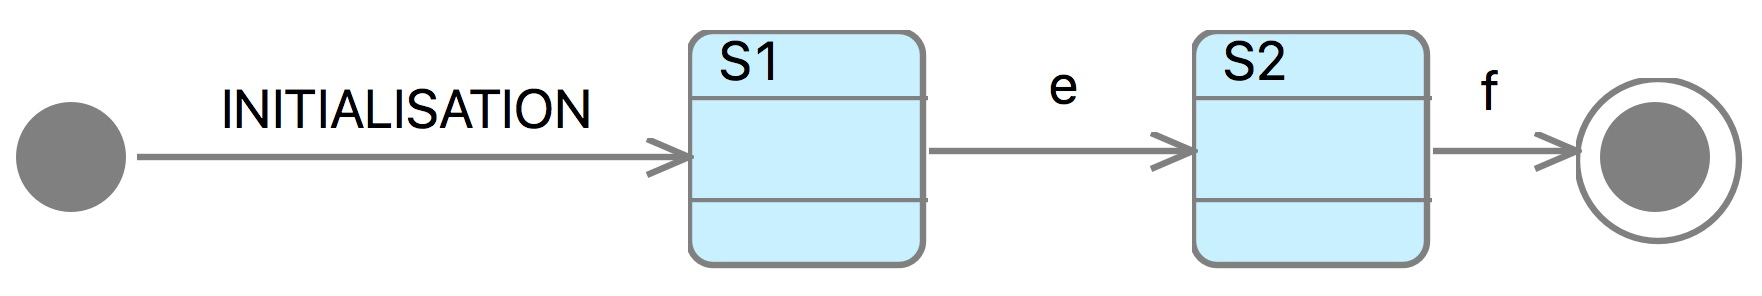
\includegraphics[width=0.6\textwidth]{figures/iumlb-SM}
% 	\caption{An example \UMLB state-machine}
% 	\label{fig:iumlb-sm}
% 	\vspace{-.5cm}
% \end{figure}

Each state is encoded as a boolean variable and the current state is indicated by one of the boolean variables being set to |TRUE|. 
An invariant ensures that only one state is set to |TRUE| at a time.
%The state-machine, is initialised by setting one state variable to |TRUE| and all others to |FALSE|.
Events change the values of state variables to move the |TRUE| value according to the transitions in the state-machine.  
% The \EventB translation%
% %
% \footnote{%
%   Here, $\mathrm{partition(S, T1, T2, \ldots)}$ means the set $S$ is partitioned into disjoint (sub-)sets $T1, T2, \ldots$.
% that cover $S$} 
% of the state-machine in Figure~\ref{fig:iumlb-sm} can be seen in Listing~\ref{lst:eventb-sm}.
% \UMLB also provides the option of an alternative translation with a single state variable ranging over an enumerated type of states, however, the boolean representation of each state is more natural for a user to reference in \SCXML guards and actions.
	
While the \UMLB translation deals with the basic data formalisation of state-machines it differs 
significantly from the semantics discussed in this manuscript. 
\UMLB adopts \EventB's simple guarded action semantics and does not have a concept of triggers and run-to-completion.
Here we make use of \UMLB's state-machine translation but provide a completely different semantic by generating a behaviour into the underlying \EventB events that are linked to the generated \UMLB transitions.
% \begin{lstlisting}[caption={Translation of the state-machine in Fig.~\ref{fig:iumlb-sm}},label={lst:eventb-sm}, language=Event-B, escapechar=|, frame=single]
% variables S1 S2
% invariants 
% 	TRUE !: {S1, S2} => partition({TRUE}, {S1}/\{TRUE}, {S2}/\{TRUE})
% events
%     INITIALISATION: begin S1, S2 := TRUE, FALSE end
%     e: when S1 = TRUE then S1, S2 ≔ FALSE, TRUE  end
%     f: when S2 = TRUE then S2 := FALSE end
% end
% \end{lstlisting}
%%% Local Variables:
%%% mode: latex
%%% TeX-master: "../main"
%%% End:

% !TEX root = ../main.tex

\subsection{SCXML}
\label{sec:scxml}

\SCXML is a modelling language based on Harel statecharts with facilities for adding data elements that are manipulated by transition actions and used in conditions for their firing. \SCXML follows the usual `run to completion' semantics of such statechart languages, where trigger events\footnote{In \SCXML the triggers are called `events', however, we refer to them as `triggers' to avoid confusion with \EventB} may be needed to enable transitions. Trigger events are queued when they are raised, and then one is de-queued and consumed by firing all the transitions that it enables, followed by any (un-triggered) transitions that then become enabled due to the change of state caused by the initial transition firing. This is repeated until no transitions are enabled, and then the next trigger is de-queued and consumed. There are two kinds of triggers: internal triggers are raised by transitions and external triggers are raised by the environment (spontaneously as far as our model is concerned). An external trigger may only be consumed when the internal trigger queue has been emptied. 

\begin{lstlisting}[caption=Pseudocode for 'run to completion',label={lst:scxml-r2c}, frame=single]
while running:
	while completion = false
		if untriggered_enabled
			execute(untriggered())
		elseif IQ /= {}
			execute(internal(IQ.dequeue)) 
		else
			completion = true
		endif
	endwhile
	if EQ /= {}
		execute(EQ.dequeue) 
		completion = false
	endif
endwhile 
\end{lstlisting}

Listing~\ref{lst:scxml-r2c} shows a pseudocode representation of the run to completion semantics as defined within the latest W3C recommendation document~\cite{scxmlwebsite}. Here IQ and EQ are the triggers present in the internal and external queues respectively. We adopt the commonly used terminology where a single transition is called a \emph{micro-step} and a complete run (between de-queueing external triggers) is referred to as a \emph{macro-step}.

%%% Local Variables: 
%%% mode: latex
%%% TeX-master: "../main.tex"
%%% End: 


%%% Local Variables:
%%% mode: latex
%%% TeX-master: "../main"
%%% End:


% !TEX root = ../SCXMLREF.tex


\section{Intrusion Detection System}
\label{sec:secbot}

An \IDS is used to illustrate the use of refinement in \statecharts and how it is supported by \EventB verification tools.
The \IDS is designed using an \ASIC which connects to a buzzer and a sensor over a \SPI bus. The system is controlled via the \ASIC on the \SPI bus. At power-up, the \ASIC sends commands over the \SPI bus to initialise the sensor and the buzzer. After waiting for 50 milliseconds the \ASIC enters its main routine, which makes the buzzer respond to the sensor. In the early design phase the \statechart model of this system may be limited to the \ASIC that captures the initialisation of the peripherals and the 50 ms wait. In the interest of simplicity, we elide all details of the main routine.

A \statechart model of this system is shown in Fig.~\ref{fig:ASIC}. The \ASIC starts by initialising the buzzer; this involves sending a message over the \SPI bus. These messages constitute an implementation detail that we elide at this abstraction level. Once the message is sent (which will be indicated by some event saying that the \SPI system is done), the \ASIC moves on to initialise the sensor. After that the \ASIC moves into a waiting state for 50 ms, and finally moves into the state which represents normal operation. \KarlaAdd{At this abstraction the} \textbf{spi\_done} \KarlaAdd{trigger, which indicates that the }\SPI \KarlaAdd{system has finished, is an internal trigger that can be fired at any time.} \KarlaDelete{At this abstraction the spi done triggered, which signals completion by the SPI system, is an internal trigger that can be fired at any time.}

In a subsequent level of refinement, shown in Fig.~\ref{fig:ASIC_SPI_1}, the designer \KarlaAdd{uses superposition refinement to} add\KarlaDelete{s} a parallel state representing the \SPI subsystem. The \SPI subsystem is usually \SonChange{on}{in} an \textbf{Idle} state until the \textbf{send\_message} trigger is raised, at which point the \SPI subsystem enters a state \textbf{Sending Message}, which represents sending the message, byte by byte. When the last byte of the message is sent, it raises the \textbf{spi\_done} trigger, allowing the other parallel state to continue, while \SonAdd{the} \SPI subsystem returns to idle. In the current refined model we have incorporated the implementation details for raising \textbf{spi\_done} and introduced a new internal trigger 
\textbf{send\_message}, which is nondeterministic at this point.

\begin{figure*}[!tb]\centering
	    \begin{subfigure}[t]{0.3\textwidth}
	        \begin{centering}
	        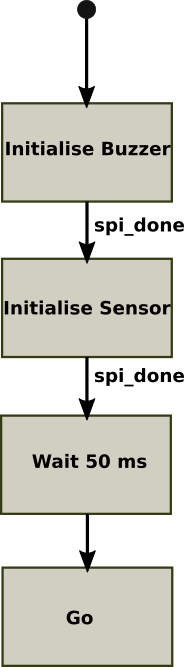
\includegraphics[height=2.5in]{figures/ASIC}
	        \caption{\ASIC component high level abstraction}
	        \label{fig:ASIC}
	        \end{centering}
	    \end{subfigure}
\qquad
	    \begin{subfigure}[t]{0.5\textwidth}
	        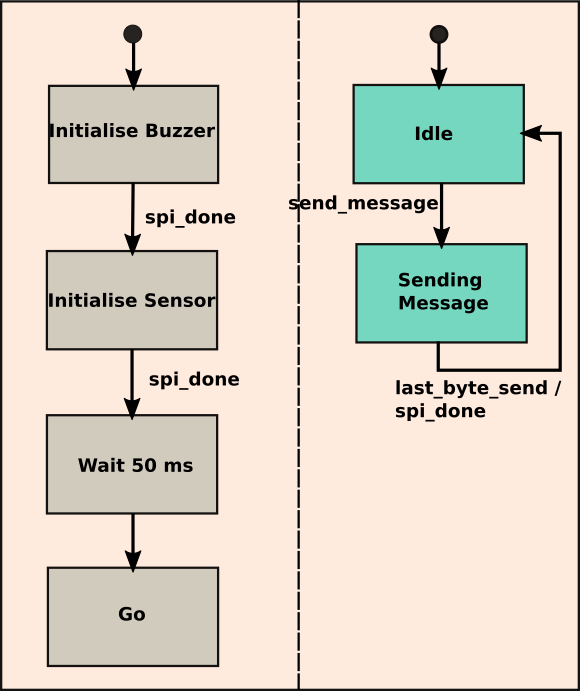
\includegraphics[height=2.5in]{figures/ASIC&SPI_1}
	        \caption{First refinement introducing the abstract model of the \SPI subsystem.}
	        \label{fig:ASIC_SPI_1}
	    \end{subfigure}
	    \caption{\Statechart diagram for \IDS including the abstract representation of the \ASIC and \SPI components.}
\end{figure*}

The model can be further refined by incorporating more details on how the initialisation states, the wait state, and the \SPI subsystem operate, including how they interact with each other. The \statechart diagram for this refinement level is in Fig.~\ref{fig:ASIC_SPI_2}. The \textbf{Initialise Buzzer} state constructs the \SPI message to send, then raises the \textbf{send\_message} trigger, and then waits.
After \textbf{send\_message} is raised, the \SPI subsystem reacts. It spins for a while in the \textbf{Send Byte} state, looping as many times as it takes to get to the last byte in the message. When the last byte in the message is sent, it goes back to \textbf{Idle} and raises an event which allows the state machine on the left to proceed. The sensor is then initialised in a very similar manner to the buzzer. After both peripherals are initialised, the state machine goes into the \textbf{Wait 50 ms} state, where it increments a counter until it reaches some maximum, then exits.

\begin{figure}[!tbp]
  \begin{centering}
  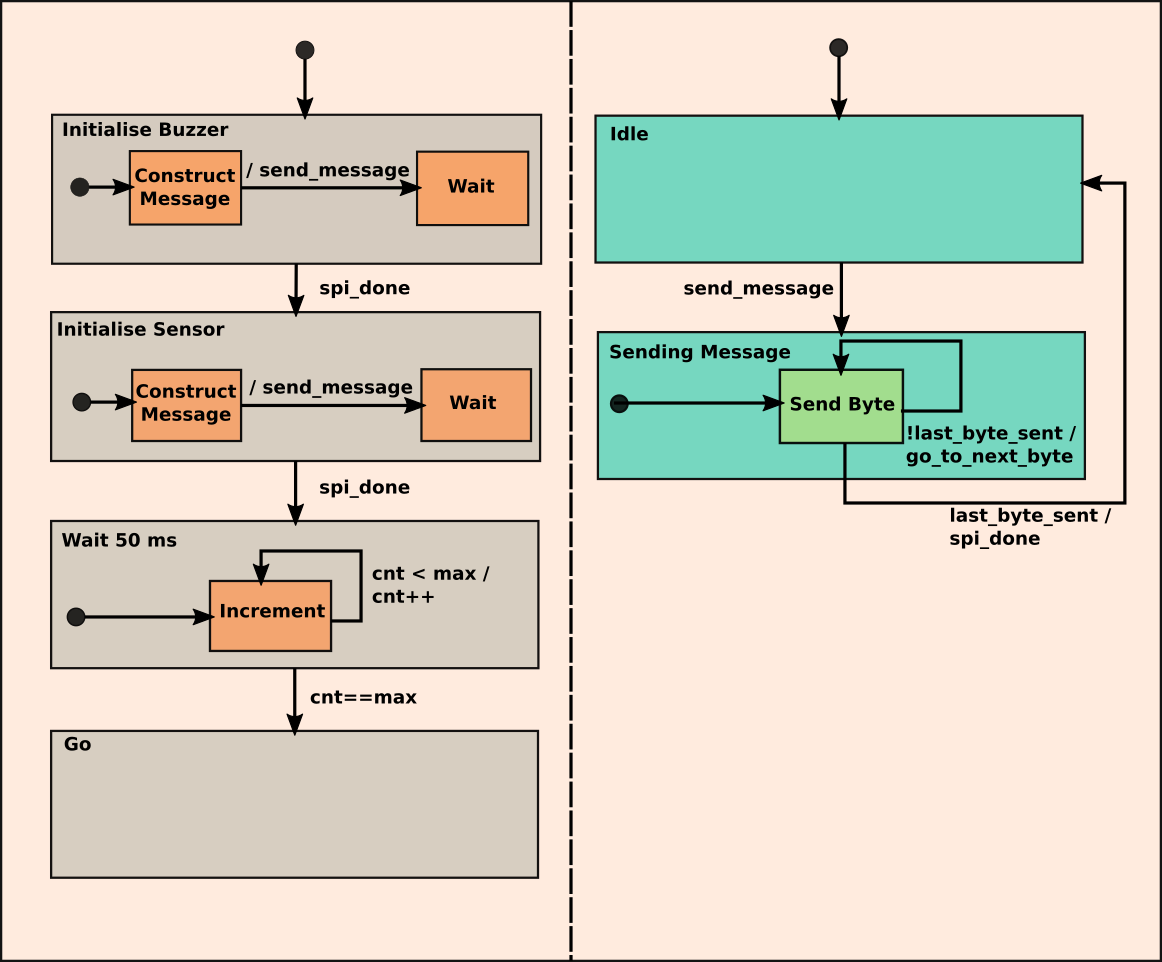
\includegraphics[width=0.8\textwidth]{figures/ASIC&SPI_2}
  \caption{\Statechart diagram for \IDS including implementation details for the messages sent between the system components.}
  \label{fig:ASIC_SPI_2}
  \end{centering}
\end{figure} 

The system described must send messages to complete the initialisation of the buzzer and sensor, but once the main routine is reached (\textbf{Go} state) no more messages should be sent through the \SPI bus. As a result, a desirable safety property is that \emph{when the \ASIC is in the \textbf{Go} state the \SPI subsystem
must be in the \textbf{Idle} state}.
\ColinChange{This safety property is introduced in the first refinement and maintained by subsequent refinements.}
{This safety property should hold from the first refinement and be preserved in all future refinements.}



%%% Local Variables:
%%% mode: latex
%%% TeX-master: "../SCXMLREF"
%%% End:



% !TEX root = ../SCXMLREF.tex

\section{Discussion}
\label{sec:discussion}

In order to introduce a notion of refinement into \SCXML we need to consider the kinds of things we would like to do in refinements and what properties should be preserved.
In practice we wish to leverage existing \EventB verification tools and hence adopt a notion of refinement that can be automatically translated into an equivalent \EventB model consisting of a chain of refinements.

While it would be possible to utilise \EventB's data refinement to perform complex refinements at the \statechart level (for example replacing an abstract \statechart with a different one in the refined model), this would lead to complex proof obligations and is impractical when the \SCXML model is a single \Statechart (rather than a chain of refined models).
We prefer to use particular refinement idioms at the \statechart level that correspond to \EventB's superposition refinement and thus have simpler proof obligations. 
These refinement idioms are very natural from an engineering perspective (as illustrated by the running example).
 Hence we start from the following requirements which allow superposition refinements and guard strengthening in \SCXML models:
\begin{itemize}
	\item The firing conditions of a transition can be strengthened by adding further textual constraints about the state of other variables and state machines in the system.
	\item The firing conditions of a transition can be strengthened by being more specific about the (nested) source state,
	\item Nested \Statecharts can be added in refinements.
	\item Ancillary data can be added and corresponding actions to alter it can be added to transitions.
	\item Raise actions can be added to transitions to define how internal triggers are raised. These internal triggers may have already been introduced and used to trigger transitions in which case they are non-deterministically raised at the abstract levels. (Note that external triggers are always unguarded and cannot be refined).
	\item Invariants can be added to states to specify properties that hold while in that state.
\end{itemize}

Refinement should preserve the value of the abstract state after each micro-step and at the end of each macro-step. The abstract state should not be altered by any new micro-steps that are introduced into an abstract macro-step, nor by any new macro-steps that are introduced. (Note that these goals take the view that macro-steps should align through refinement. An alternative approach that we are considering for future work takes the view that the macro-steps need not align and a micro-step may shift from one macro-step to another in a refinement). 

There is an inherent difficulty with refining `run to completion' semantics which require that every enabled micro-step is completed before the next macro-step is started. The problem is that, in a refinement, we want to strengthen the conditions for a micro-step. However, by making the micro-steps more constrained we may disable them and hence make the completion of enabled ones more easily achieved. This makes the guard for taking the next macro-step weaker breaking the notion of refinement.

While it is always possible to abstract away sufficiently to reach a common semantics (see~\cite{Snook12:FMCO} for example), in this work we wish to explore verification that considers `run to completion' behaviour as closely as possible.    
To simulate the `run to completion' semantics in \EventB, we initially adopted a scheduler approach where `engine' events decide which user transitions should be fired based on their guards. 
Boolean flags are then used to enable these transitions which must then fire before the next step of the engine.
The engine implements the operational semantics of Listing~\ref{lst:scxml-r2c} by deciding when to use internal or external triggers.
To allow for transition guards to be strengthened in later refinements the scheduling engine may continue without actually firing the transitions.
However, this introduces many additional behaviours making simulation difficult.
We abstract away from the \SCXML rules about executing parallel transitions in document order and adopt non-deterministic firing order of transitions. 
A consequence is that if transitions that can fire in parallel assign to the same variable as each other the resulting value is non-deterministic.
%\ColinInlineCommented{Son's suggestion to move the non-determinism to the enabling step may improve this scheduler engine approach}

Due to difficulties with non-deterministic firing of user transitions we developed an alternative approach where a separate event is generated for each combination of transitions that could possibly be fired together in the same step. 
For example, if T1 and T2 are transitions that could both become enabled at the same scheduler step, four events are needed to cater for the possible combinations: neither, T1, T2 and both (where the combined event is constructed from the conjunction of guards and parallel firing of actions). 
To allow for strengthening of the guards  in refinement we omit the negation of guards
%(if $Gref \implies Gabs$  it does not follow that $\neg Gref \implies \neg Gabs$) 
leaving the choice of lesser combinations, including the empty one, non-deterministically available in case of future refinement.
For example, T1 could fire alone even if T2 is enabled since we cannot add the negation of T2's guard to T1 unless we know that it will never be strengthened. 
For future work we may consider extending \SCXML with an attribute to indicate that a guard is \emph{finalised} so that the negation can be used.

With this approach, since there is only ever a single event to be fired, the scheduler can be integrated with the events that represent the transition combinations, greatly simplifying the Event-B model.
Instead of explicit events to progress and implement the scheduling engine, an abstract machine is provided with events that can be refined by the translation of the user's \SCXML model.
This has benefits both for animation which is easier to follow having less translation artefacts and for proof where the obligations are directly associated with particular transition combinations. 
Another benefit is that any parallel assignments to the same variable are rejected by the Event-B static checker.
The disadvantage, of course, is that there could be a combinatorial explosion in the number of events generated.
In practice though, this is unlikely since the number of parallel state machines is usually quite small.
So far our examples have required few or no parallel transitions.




%% !TEX root = ../SCXMLREF.tex

\section{Extensions to \SCXML}
\label{sec:extensions}
 
The following syntax extensions are added to \SCXML models to support refinement and invariant verification. 
Note that it would be possible to avoid these annotations using an approach where an entirely different model is constructed for each refinement level (as in \EventB).
However, we wished to retain the current \SCXML modelling approach where a single copy of the model is developed. To do so with superposition refinement requires a means of indicating the intended refinement level of each part of the model and a mechanism for expressing constraint predicates to be verified.
% features needed in \iUMLB/\EventB. These extensions are prefixed with `iumlb:' in order to distinguish them for the \SCXML XML parser. (So that they are ignored by \SCXML simulation tools). 
%They are loaded by EMF as generic feature maps (‘Any’ for contained elements and ‘AnyAttribute’ for attributes).
\begin{itemize}
	\item \textbf{refinement} - an integer attribute representing the refinement level at which the parent element should be introduced (see Listing~\ref{lst:secBot}, line~\ref{line:refinement}).
	\item \textbf{invariant} - an element that generates an invariant in \iUMLB. This provides a way to add invariants to states so that important properties concerning the synchronisation of state with ancillary data and other state machines can be expressed (see Listing~\ref{lst:secBot}, line~\ref{line:invariant}).
	\item \textbf{guard} - an element that generates a transition guard in \iUMLB. 
	This provides a way to add new guard conditions to transitions over several refinement (Listing~\ref{lst:secBot}, line~\ref{line:guard}) as well as providing an element with attributes such as derived (for \EventB theorems), name and comment.
	\item \textbf{predicate} - a string attribute used for the predicate of a guard or invariant (Listing~\ref{lst:secBot}, line~\ref{line:predicate}).
\end{itemize}
%Other attributes added for \iUMLB elements are: \textbf{iumlb:name}, \textbf{iumlb:derived}, \textbf{iumlb:type}, \textbf{iumlb:comment}.

\begin{lstlisting}[caption={\textbf{Wait50ms} state snippet of \SCXML model representation illustrating the use of different \SCXML modeling features, as well as, added syntax extensions},label={lst:secBot}, language=xml, escapechar=|, frame=single, float=t]
...
<state id="Wait50ms" iumlb:refinement="2">
	<initial iumlb:refinement="2"> |\label{line:refinement}|
		<transition cond="cnt=0" target="Increment"/> 
	</initial>
	<iumlb:invariant name="check_cnt" iumlb:predicate="cnt &lt; max" iumlb:refinement="2"/> |\label{line:invariant}|
	<transition cond="" target="Go" iumlb:refinement="0" />
	<state id="Increment" iumlb:refinement="2">
		<transition cond="" event="tick" target="Increment">
			<assign attr="cnt" expr="cnt+1" location="cnt"/>
			<iumlb:guard name="stillCounting" iumlb:predicate="cnt &lt; 5"/> |\label{line:predicate}|
		</transition>
		<transition cond="" target="WAITDone">
			<iumlb:guard name="doneCounting" iumlb:predicate="cnt = 5"/> |\label{line:guard}|
    	</transition>
	</state>
	<final id="WAITDone" iumlb:refinement="2"/>
	<datamodel>
		<data expr="0" id="cnt" src="" iumlb:type="NAT "/>
	</datamodel>
</state>
...
\end{lstlisting}

%Hierarchical nested state charts are translated into similarly structured \iUMLB state-machines. The generated \iUMLB model contains refinements that add nested state-machines as indicated in the  \SCXML \statechart (see Listing~\ref{lst:secBot}) by the \textbf{iumlb:refinement} attributes annotated on state elements. \iUMLB transitions are generated for each \SCXML transition and linked to \EventB events that represent each of the possible synchronisations that could involve that transition.


%%% Local Variables:
%%% mode: latex
%%% TeX-master: "../SCXMLREF"
%%% End: Now in discussion

% !TEX root = ../main.tex

\section{\SCXML Translation to \UMLB/\EventB}
\label{sec:translation}

The translation of a specific \SCXML model to \UMLB and  \EventB, comprises the following stages: 
\begin{itemize}
	\item 
Firstly, a basis machine and context are created to embody the semantics of the \SCXML language (as described in Section~\ref{sec:run-completion}).
The basis provides variables and events to model the queue of triggers as well as abstract versions of events to model transitions firing.
The basis is independent of the particular \SCXML model which is added in subsequent refinements.
Hence it is not necessary to re-prove any of the proof obligations associated with this basis.
	\item 
Secondly, all possible combinations of each set of transitions that can fire together are calculated and corresponding events are generated, at appropriate refinement levels (given by the refinement annotations embedded in the \SCXML model), that refine the abstract basis events.
The transitions that can fire together are those that are triggered by the same trigger (or are both untriggered) and are in different parallel (`and') sub-states.
If these transitions raise internal triggers, a guard, |{i1, i2, ...} <: content(raisedTriggers)| (where |i1, i2, ...| have been added to the internal triggers set), is introduced to define the raised triggers parameter. 
The subset used in the guard retains non-determinism to allow more triggers to be raised in later refinements.
For triggered transitions, the trigger is specified by a guard that defines the value of the trigger parameter. 
	\item 
Thirdly, at each refinement level, the \SCXML state-chart is translated into a corresponding \UMLB state-machine whose transitions elaborate (i.e. add state change details to) the transition combination events that the transition may be involved in.
A transition may fire in parallel with transitions of parallel nested state-machines that have the same (possibly null) trigger.
	\item
Finally the \UMLB state-machine is translated into \EVENTB by programmatically invoking the \UMLB translator.
\end{itemize}

% Further details of the translation are given in~\cite{MoSn16,MoSnHo18,MoSnHo-ABZ2020}.

 A previous version of the translator was described in ~\cite{MoSnHo18} New features of the translation added since~\cite{MoSnHo18} are as follows:
 \begin{description}
 \item[Trigger queues in basis:]
 	\begin{sloppypar}
 		The encoding of trigger queues in the abstract basis context and machine has been improved so that a queue is properly modelled as a sequence of triggers.
 		This more accurately reflects the \SCXML semantics.
 	\end{sloppypar}
 \item[Dequeing triggers from queues:]
   \begin{sloppypar}
     The abstract basis machine has been improved so that triggers are properly dequeued before potential use,
     which allows triggers to be discarded if the controller cannot respond to them. 
     This more accurately reflects the \SCXML semantics and was necessary in order to model the new drone case study properly.
   \end{sloppypar}

 \item[Finalisation:] Transitions can be flagged as finalised which means their guards can not be strengthened in subsequent refinements. This allows them to `enforced' when they are enabled (i.e. completion cannot occur until they have fired) which is needed for verification. 

 \item[Restricted raising of internal triggers:] Once a trigger is introduced it must immediately be raised at that refinement level by any transitions that wish to do so. It cannot be raised in later refinements except by newly introduced transitions. This restriction was necessary to make simulation more useful by removing non-deterministic raising of triggers in anticipation of refinements.

 \item[Context instantiation:] The axioms of the basis context, that allow future triggers to be added, has been improved so that \PROB\footnote{ProB is an animator, constraint solver and model checker for the B-Method. https://www3.hhu.de/stups/prob} can automatically create an instantiation. 

 \end{description}

A tool to automatically translate \SCXML source models into \UMLB has been produced. 
The tool is based on the \EMF and uses an \SCXML meta-model provided by Sirius~\cite{siriuswebsite} which has good support for extensibility. 
The \UMLB state-machine is subsequently translated into \EVENTB using the standard \UMLB translation which provides variables to model the current state and guards and actions to model the state changes that transitions perform.
% Further details of the translation are given in~\cite{MoSnHo18,MoSnHo-ABZ2020}.

Figure~\ref{fig:drone2UMLB} shows the UML-B model of the drone at refinement level 2 (equivalent to Figure \ref{fig:drone4} without the detail inside TAKEOFF).
The structure of the state-machine is similar to the \SCXML version with purple shading indicating the previously added states and light blue shading indicating the detail added at this refinement level.
State invariants (properties that should hold while that state is active) are shown in |TAKEOFF|, |FLY| and |BATTERYOK|.
Verification of these invariants is discussed in Section~\ref{sec:verificationSafety}.

\begin{figure}[]
%	\vspace{-.4cm}
	\centering
	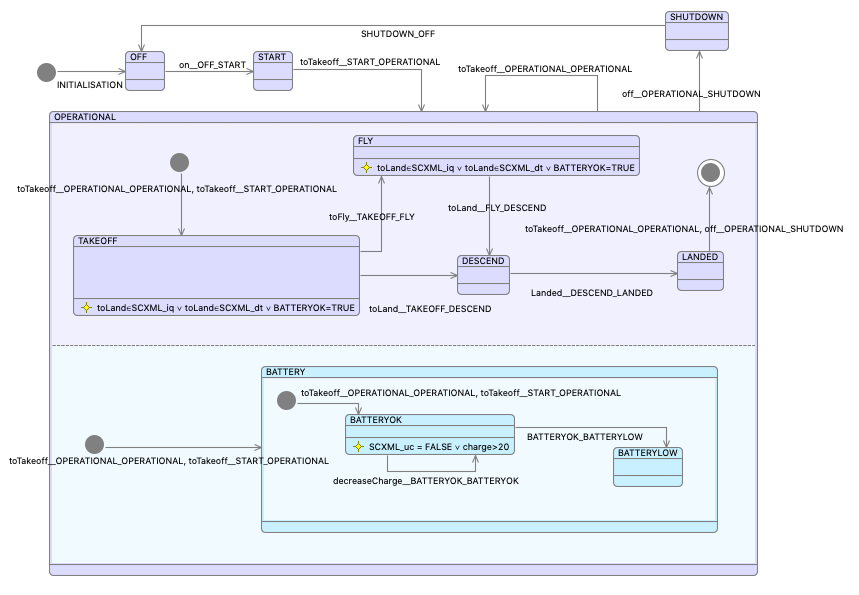
\includegraphics[width=0.90\textwidth, trim=0 40 0 0]{figures/drone2UMLB.png}
	\caption{Generated UML-B State-machine for drone refinement level 2. }
	\label{fig:drone2UMLB}
%	\vspace{-.4cm}
\end{figure} 

%%% Local Variables:
%%% mode: latex
%%% TeX-master: "../main"
%%% End:

% !TEX root = ../SCXMLREF.tex

\section{Verification of Intrusion Detection System}
\label{sec:example}

One of our main goals is to express properties in \SCXML intermediate refinements and prove them via translation to \EventB.
In this section we illustrate how this can be done in the \IDS example.

Properties about the synchronisation of parallel state-machines (such as |Go = TRUE => Idle = TRUE|)
% and |ASIC=Wait50ms => SPI=IDLE|
can be difficult to verify for all scenarios via simulation in \SCXML. 
Proof of such properties is a major benefit of translating into Event-B.  
Furthermore,  in order to benefit from the abstraction provided by Event-B, we would like to prove such things at abstract levels before the complication of further details are introduced. 
Typically these further details concern the raising of internal triggers that contribute to the synchronisation we wish to verify. 
Therefore additional constraints, that are an abstraction of the missing details, are needed about triggers in order to perform the proof.
% \begin{figure}[!tbp]
\begin{figure}[!h]
	\vspace{-.4cm}
	\centering
	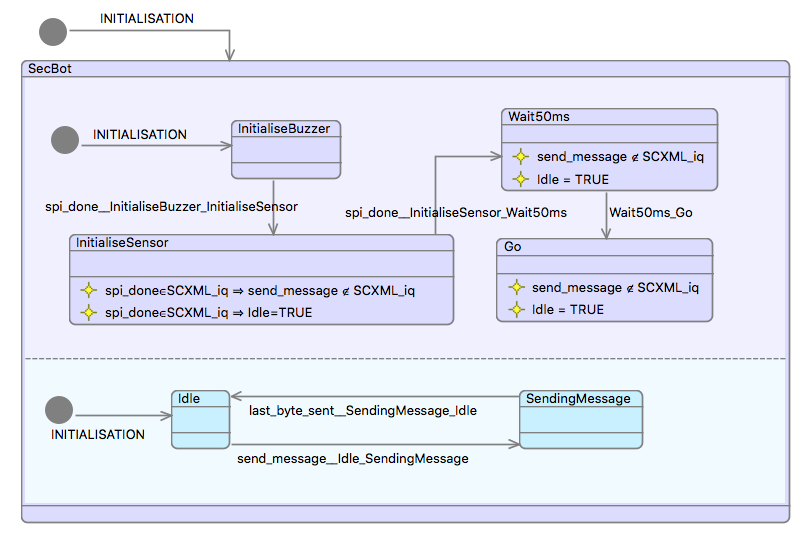
\includegraphics[width=0.8\textwidth]{figures/iumlb_verif}
	\caption{State invariants to be verified at refinement level 1.}
	\label{fig:iumlb-verif}
	\vspace{-.4cm}
\end{figure}

Fig.~\ref{fig:iumlb-verif} is the generated \iUMLB showing state invariants (textual properties with a star icon inside states) to be verified. Note that the invariants are added to the \SCXML model but are easier to visualise in the \iUMLB with the current tooling.
The main aim is to show the property |Idle=TRUE| holds in state |Go|. 
This is true because after sending the message while in |InitialiseSensor|, no other messages are triggered by the |ASIC|, so the |SPI| subsystem stays in the |Idle| state indefinitely. 
To enable the provers to discharge the proof obligation we work back along the |ASIC|'s sequence of states. 
That is, |Idle = TRUE| is maintained in state |Go| if it holds in state |Wait50ms| and no |send_message| triggers are raised by the entry transition |Wait50ms_Go| nor once the |ASIC| subsystem is in state |Go|. 
To ensure this we add a guard |send_message /: SCXML_raisedTriggers| to |Wait50ms_Go| to prevent any future refinement from raising the trigger |send_message|.
(Currently, this is added verbatim but we envision a `doesn't raise' notation to avoid the user having to reference the translation artefact, |SCXML_raisedTriggers|).
We also need to prevent any future transitions from raising this trigger in the state |Go|.
To automate this for all abstract `future' events, they could be automatically generated and added to satisfy all user invariants concerning the raising of internal triggers regardless of whether they are violated in future levels. 
For example, the guard  |Go = TRUE => send_message /: SCXML_raisedTriggers| needs to be automatically added to the three `basis' events,
\ColinComment{changed `SCXML future...TransitionSet' to `SCXML futureUntriggeredTransitionSet, SCXM futureInternalTransitionSet and SCXML futureExternalTransitionSet'}
 |SCXML_futureUntriggeredTransitionSet|, |SCXML_futureInternalTransitionSet| and |SCXML_futureExternalTransitionSet| to prove they do not break the property being verified. 
If it is not obeyed by future transitions, guard strengthening proof obligations will fail, making it obvious where the problems lie.
As indicated above, we now need to prove by similar means that |Idle=TRUE| holds in state |Wait50ms|. 
In this case, however, we can only say that |Idle=TRUE| in state |InitialiseSensor| after the \SPI-system finishes sending the message and raises the trigger, |spi_done|. 
Hence the state invariant for |InitialiseSensor| becomes |spi_done∈SCXML_iq => Idle=TRUE|. 
In order to prove this we again need a corresponding state invariant about |send_message| and need to make sure that the |SPI| system will never raise |send_message|.
We also ensure it does not raise |spi_done| until it is finished. 
With these invariants and additional guards the Rodin automatic provers are able to prove all proof obligations and hence verify that the |SPI| system remains in |Idle| after servicing the `Initialise Sensor' message.

In order to prove properties at an abstract level we constrain the behaviour to be added in later refinements. 
For example, we needed to add a guard to specify that a transition does not raise a particular trigger in any future refinement. 
The abstract constraints should not appear in later refinements when the details have been finalised. To do this we could introduce ranges into our refinement attributes.

%%% Local Variables:
%%% mode: latex
%%% TeX-master: "../SCXMLREF"
%%% End:

\section{Conclusion}

In conclusion ...

\begin{footnotesize}
%\begin{scriptsize}
	\vspace{6 pt}
	\noindent
	All data supporting this study are openly available from the University of Southampton repository at
	%https://tinyurl.com/SCXML-REF    \textbf{(DOI FOR FINAL)}
	\url{https://doi.org/10.5258/SOTON/D0693}

%\end{scriptsize}
%\begin{footnotesize}
\vspace{6 pt}
\noindent
\textbf{Acknowledgment:} The authors would like to thank Jason Michnovicz for developing the \IDS example used throughout the manuscript.

\par

\end{footnotesize}
%\end{scriptsize}

\bibliographystyle{plain}
\bibliography{SCXMLREF}

\end{document}

%%% Local Variables: 
%%% mode: latex
%%% TeX-master: t
%%% End: 